\section{Data Acquisition}
\label{sec:dataAcquisition}

The prediction is based on occupancy data gathered in a metro station. First some facts regarding the metro station will be given. Subsequently the data acquisition will be explained.

\subsection{Station}
\label{subsec:station}

In this section the "station" is described. First the word "station" in the area of metro networks needs to be defined.

A metro network is composed by one or more metro lines. Each line has a fixed railway with a given number of stops to allow people to get on or off the trains by means of a platform: each of these stops is called "line station". A "metro station" is the concept that represents the point in space through which a passenger gets underground and into a line station. Metro station and line station can be the same physical entity, but it is possible that there are some "metro stations" that receive two or more "metro lines" in different platforms, and have therefore, two or more "line stations" within.

The data, used in this work, are gathered in line station in Passeig de Gr\`{a}cia - Line~3~(PdG-L3) in Barcelona. Passeig de Gr\`{a}cia~(PdG) is a station in the metro network of "Transports Metropolitans de Barcelona"~(TMB) and lies in a very iconic and touristic part of Barcelona. Some of the most popular buildings designed by Antoni Gaudi are in the proximity (Casa Batll\`{o}, Casa Mil\`{a}), as well as the city's most renown and exclusive boutiques.
The metro station is a historic icon of the Barcelona metro network. First opened in December of 1924, as a (line) station for Line~3, nowadays PdG holds three different line stations: L2, L3, and L4. The stations were built in three different periods and using different construction technologies in each of the premises (contemporary to the building periods). All line stations station has been refurbished a few times since 1924 and new equipment has been added recently.

Depending on the weekday PdG is open 19~hours, 21~hours or 24~hours. Between Monday and Thursday PdG service starts at 5:00 and ends at 24:00 (19~hours). Friday service starts at 5:00 and ends at 2:00 (21~hours). On Saturday service starts at 5:00 to but remain the entire night until midnight on Sunday.

Passeig~de~Gr\`{a}cia - Line~3~(PdG-L3) turns out to be representative for many station within TMBs metro network~\cite{TMB}. Moreover PdG-L3 is a crowded station which have low-rate usage hours as well. This provides a wide range of data which allows to test with very busy peak hours as well as with off-peaks. Figure~\ref{fig:PdG-L3_platforms} depicts the platforms of PdG-L3.

\begin{figure}[htb]
  \centering
  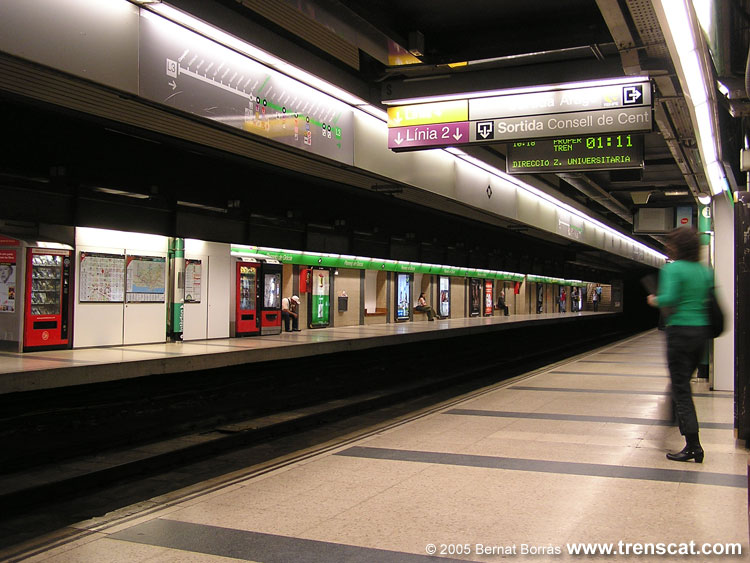
\includegraphics[width=\linewidth]{PdG-L3_platforms.jpg} 
  \caption{PdG-L3 Plattforms. \cite{TMB}}
  \label{fig:PdG-L3_platforms}
\end{figure}

The line station PdG-L3 consists of several public spaces: halls, transit areas, accesses to the platforms, and platforms. Furthermore there are private spaces such as technical rooms or staff dependencies. The private spaces are not part of the investigation in this work. Figure~\ref{fig:PdG-L3_schematic} depicts the line station schematic where the accesses to platforms are highlighted in red.

\begin{figure}[htb]
  \centering
  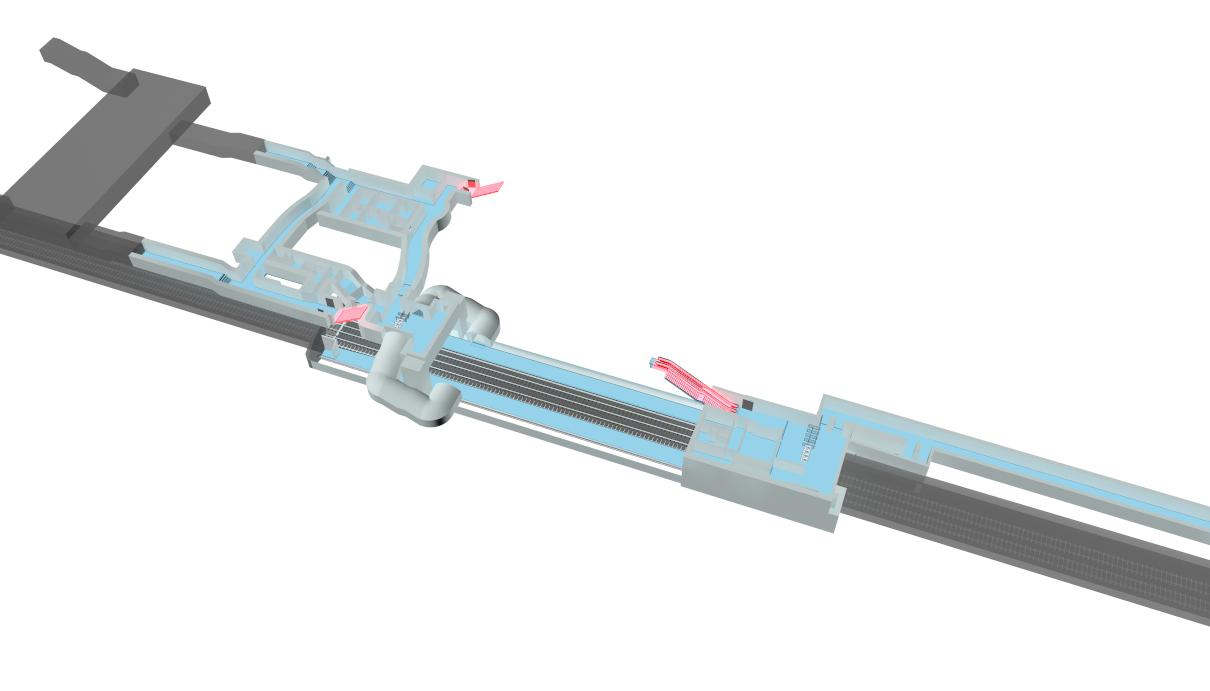
\includegraphics[width=\linewidth]{PdG-L3_schematic.jpg} 
  \caption{Schematic representation of PdG-L3. The accesses to platforms are highlighted in red. \cite{TMB}}
  \label{fig:PdG-L3_schematic}
\end{figure}

The public spaces are equipped with a Closed Circuit Television~(CCTV) for security reasons. The cameras of the CCTV-system provide images which contains the information how many people are on a dedicated time on a dedicated place. To gather these information the images needs to be processed. In the following the processing of the camera images is described in short.


\subsection{Passenger density data}
\label{subsec:PassengerDensityData}

Throughout the station a CCTV surveillance system already exists. 22~CCTV~cameras are in place where each camera provides in a circuit design subsequently the images. The images provided by each CCTV-camera are stored on a video recorder. A crowd density estimator processes the images and returns the number of passengers on this image. The number of passenger as well as date, time and the camera-ID are saved in a database.

For different reasons, e.g. bad camera picture or network errors it is possible that the image processing fails. In this case the error value "-1" is saved in the database.

The process images are not saved for privacy reasons. Figure~\ref{fig:CCTVimageProcessing} depict the processing chain.

\begin{figure}[htb]
  \centering
  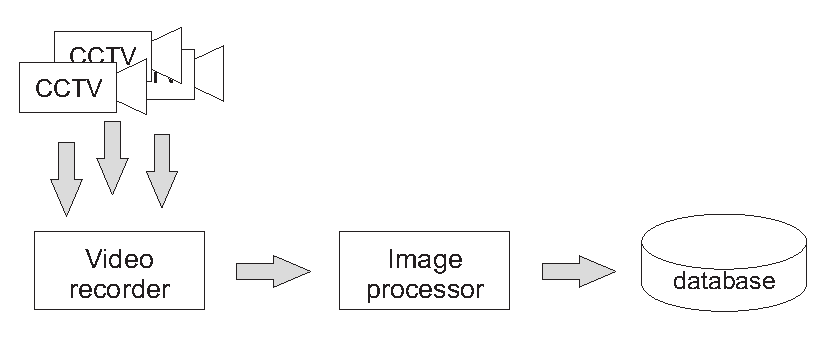
\includegraphics[width=\linewidth]{imageProcessing.pdf} 
  \caption{Gathering number of people out of the camera images.}
  \label{fig:CCTVimageProcessing}
\end{figure}

The CCTV and image processing runs 24~hours, 7~days a week. Each day 31680~datasets are saved to the database. Overall the database contains 90~days of data.
Figure~\ref{fig:rawData_week} illustrates exemplary the available values of a week. At a more detailed view of a day the service times are visible (Figure~\ref{fig:rawData_day}).

%\onecolumn
\begin{figure*}[tb]

  \centering

  \subfigure[Passenger density distribution of one camera during one week.] {
    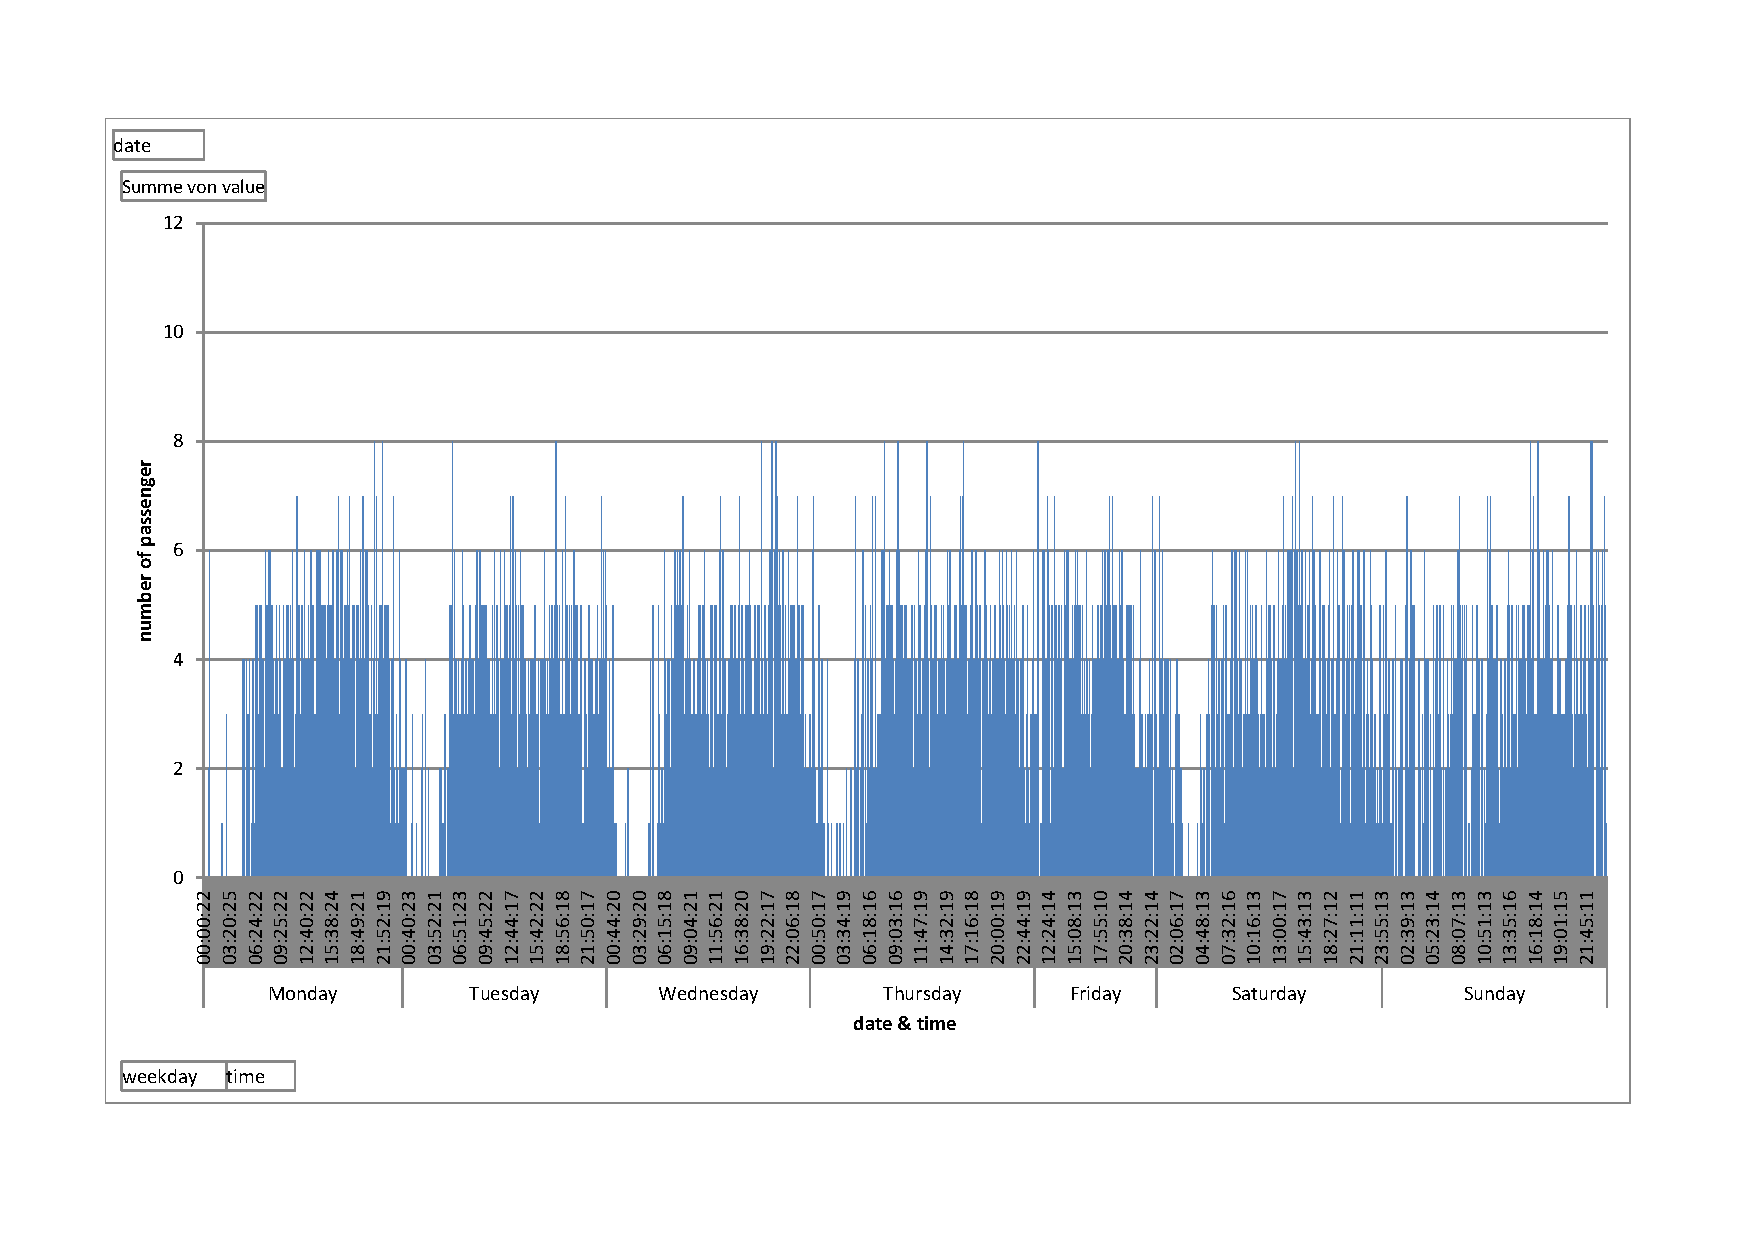
\includegraphics[width=0.46\textwidth]{rawData_week.pdf}
    \label{fig:rawData_week}
  }
  \hfill
  \subfigure[Passenger density distribution of one camera during one day.] {
    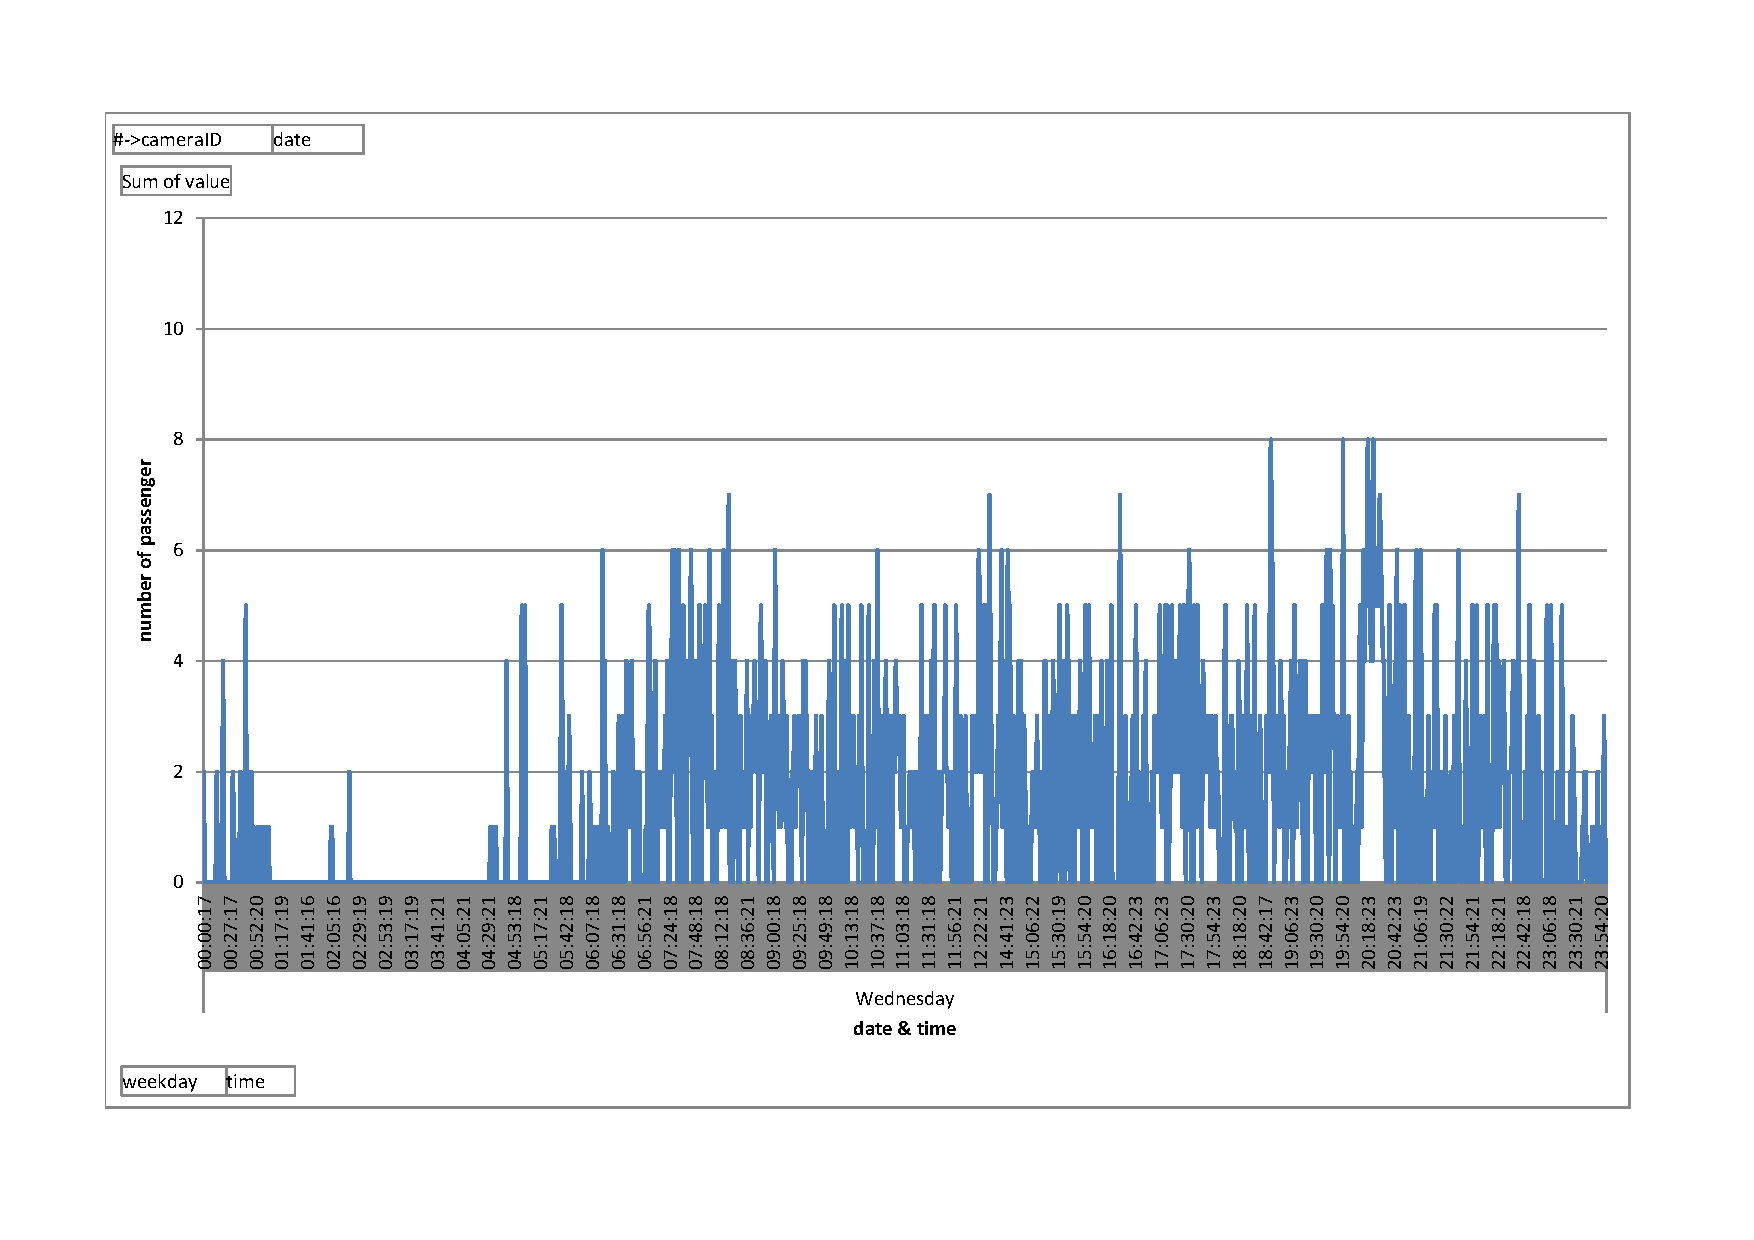
\includegraphics[width=0.46\textwidth]{rawData_day.pdf}
    \label{fig:rawData_day}
  }

  \caption{Passenger density distribution of one camera.~\cite{TMB}.}
  \label{fig:rawData}

\end{figure*}


This database of passenger density information are the base for the investigations in this paper.
